\section{Design choices}
\label{sec:design}

\subsection{Different False Attempts or Starts}
\begin{itemize}
\item Pulse based echo selection and finding or Echo-sorting (Too much direct path impact).
\item Angle-of-arrival calculation (Too less number of mics and sine based or CIR based phase measurement won't work due to high level of multi-path).
\item MUSIC based peak selection (Prior knowledge of number of peaks).
\end{itemize}

\subsection{FMCW based observations}

\subsubsection{Resolution}
It depends upon the bandwidth used.

\begin{figure}[hbt]

\centering{
\subfigure[4KHz]{
    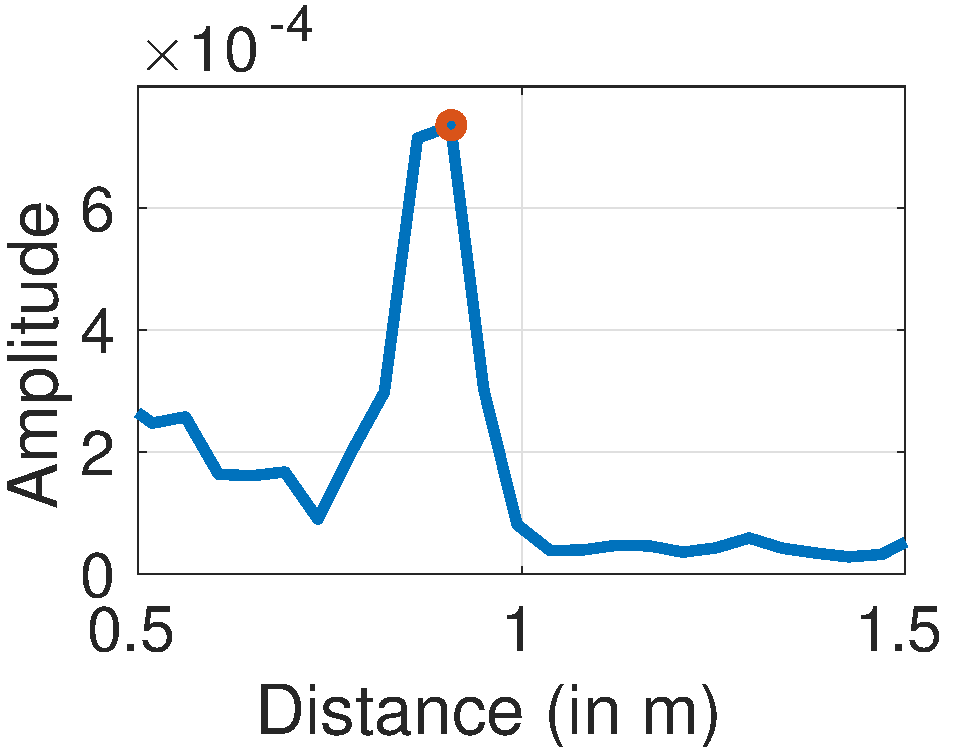
\includegraphics[width=0.46\columnwidth, keepaspectratio]{figs/4K.pdf}
    \label{fig:4K}
}
\subfigure[10 KHz ]{

    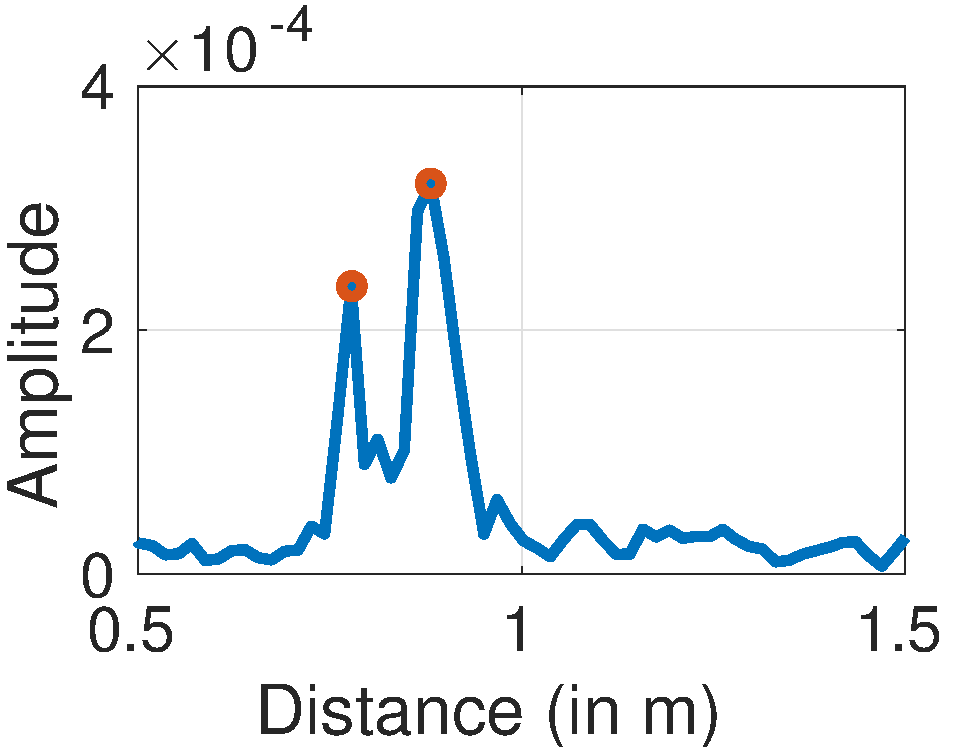
\includegraphics[width=0.46\columnwidth,  keepaspectratio]{figs/10K.pdf}
    \label{fig:10K}

}
%\vspace{-0.15in}
\caption{Impact of different bandwidths on resolution FMCW based distance measurement}
%\vspace{-0.15in}
\label{fig:resolution}
}
\end{figure}

\subsubsection{Volume Level}
It depends upon the proper volume level used.


\begin{figure}[hbt]

\centering{
\subfigure[Amplitude]{
    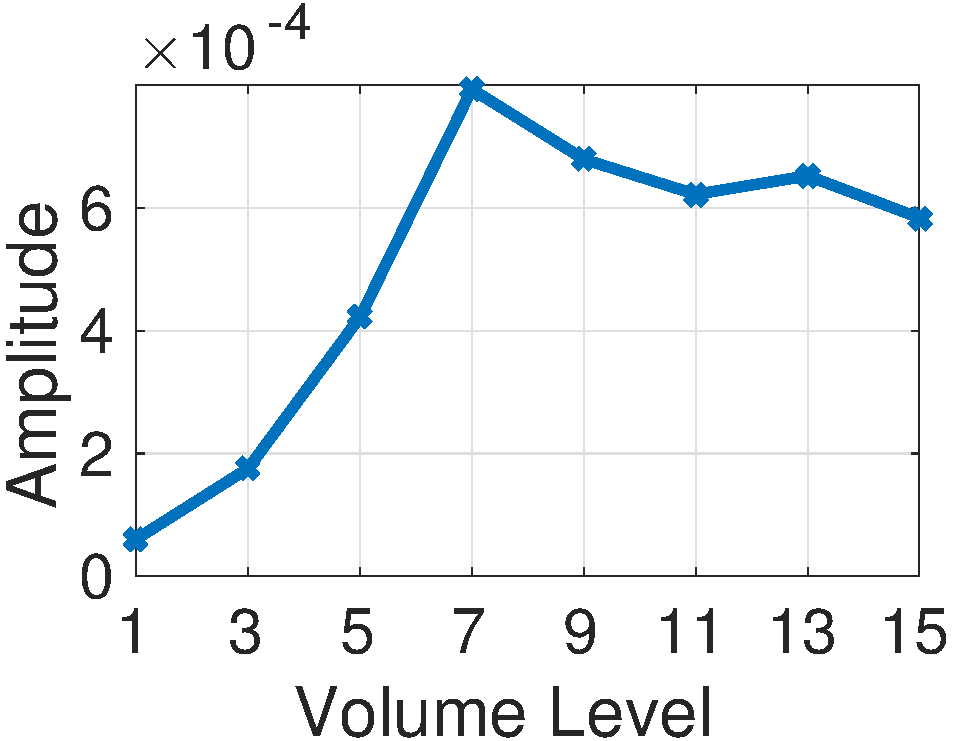
\includegraphics[width=0.46\columnwidth, keepaspectratio]{figs/volume-amp.pdf}
    \label{fig:amp}
}
\subfigure[SNR]{

    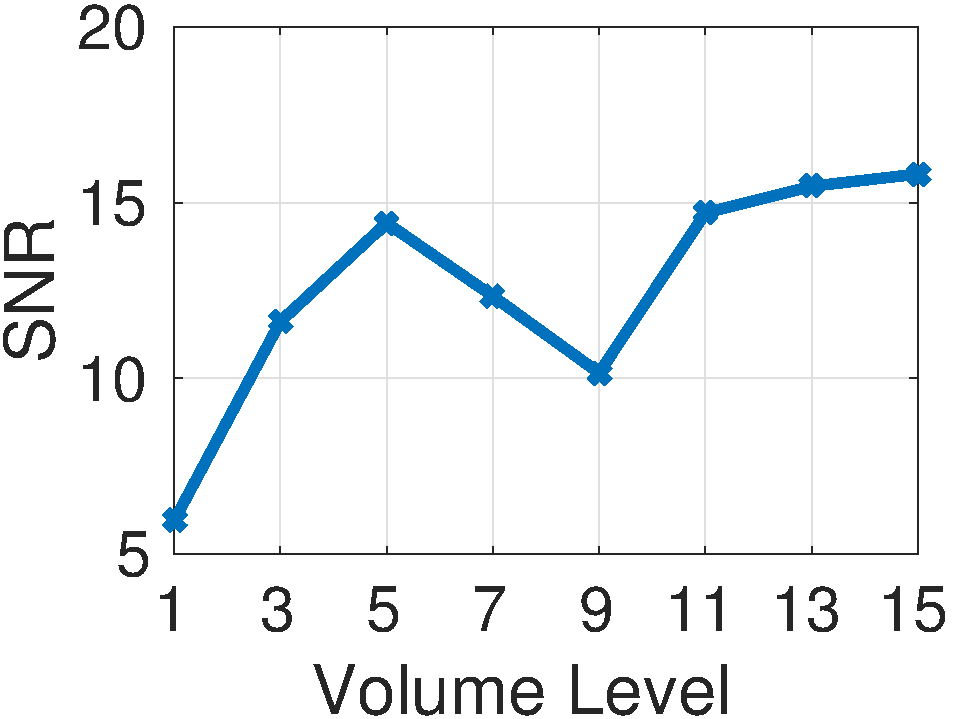
\includegraphics[width=0.46\columnwidth,  keepaspectratio]{figs/volume-snr.pdf}
    \label{fig:snr}

}
%\vspace{-0.15in}
\caption{{Impact of different volume level on FMCW based distance measurement}
%\vspace{-0.15in}
\label{fig:volume}
}
}
\end{figure}

\subsubsection{FMCW distance measurement with sizes}
It depends upon the reflection measurement with sizes.

\begin{figure}[h!t]
%\vspace{-0.1in}
\center{
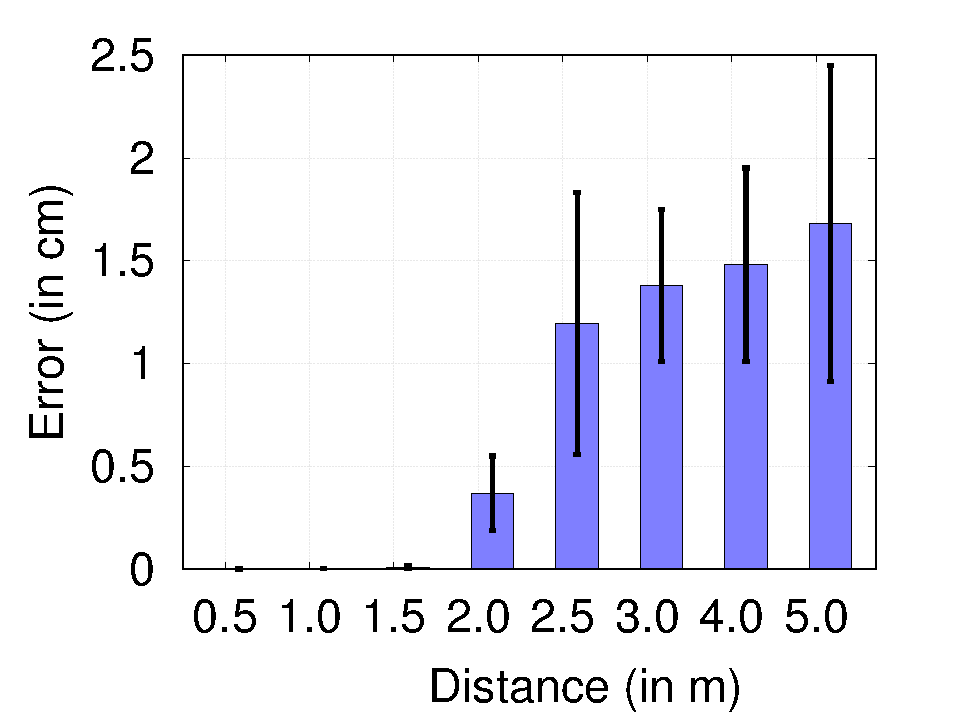
\includegraphics[width=\columnwidth]{figs/distance_error.pdf}
%\vspace{-0.1in}
\caption{FMCW error change with distance}
%\vspace{-0.1in}
\label{fig:distance_error}
}
\end{figure}

\begin{figure}[h!t]
%\vspace{-0.1in}
\center{
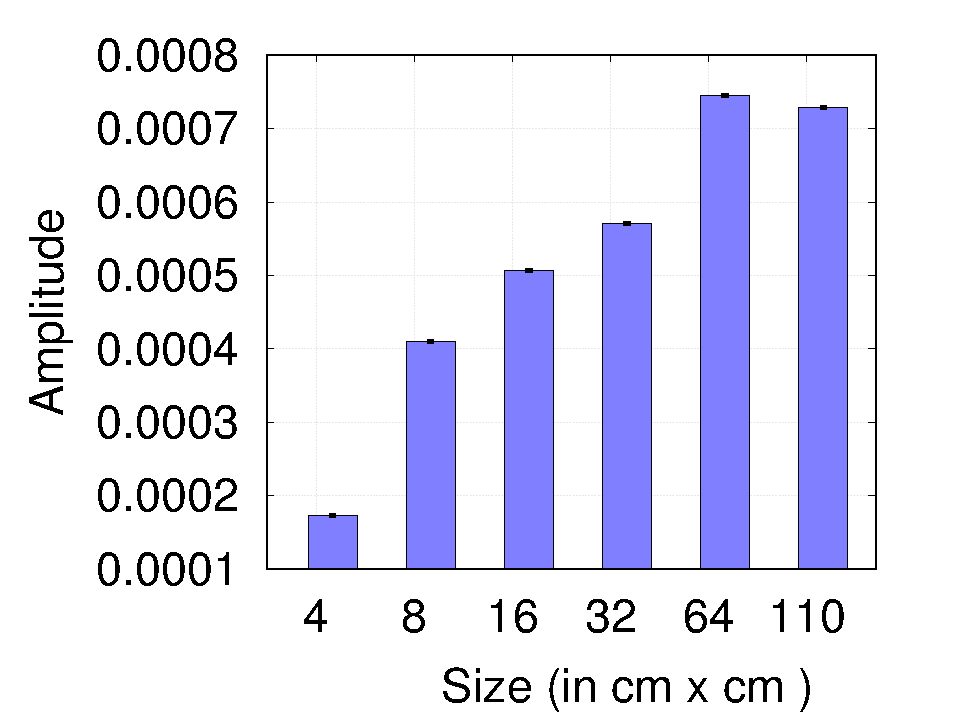
\includegraphics[width=\columnwidth]{figs/size_error.pdf}
%\vspace{-0.1in}
\caption{FMCW amplitude with different sizes}
%\vspace{-0.1in}
\label{fig:size_error}
}
\end{figure}

\begin{figure}[h!t]
%\vspace{-0.1in}
\center{
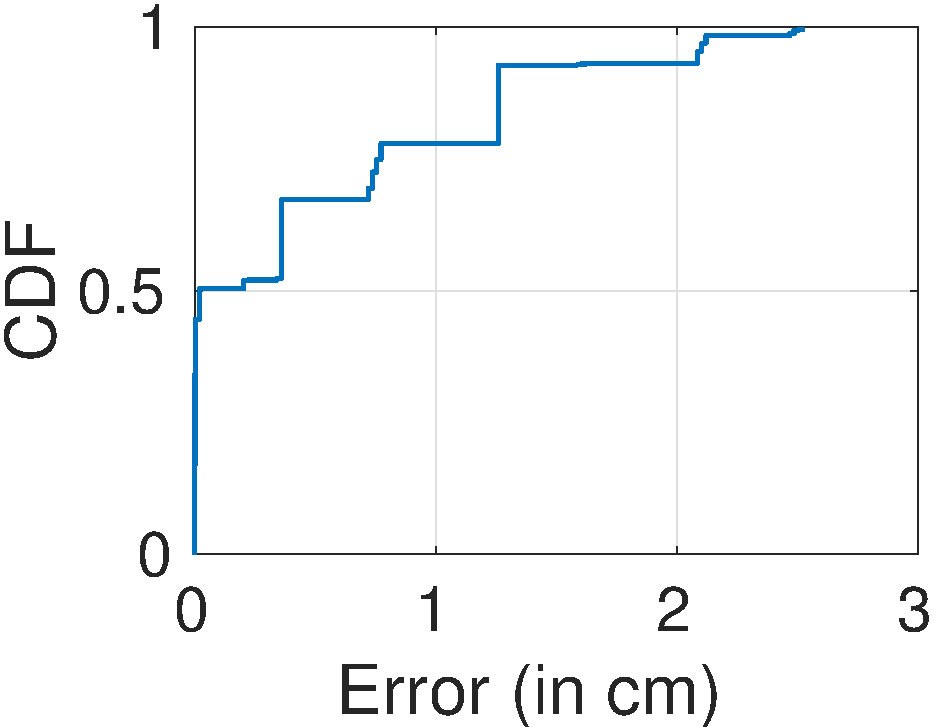
\includegraphics[width=\columnwidth]{figs/cdf-localization.pdf}
%\vspace{-0.1in}
\caption{{\small CDF}}
%\vspace{-0.1in}
\label{fig:cdf}
}
\end{figure}
\begin{figure}[h!t]
%\vspace{-0.1in}
\center{
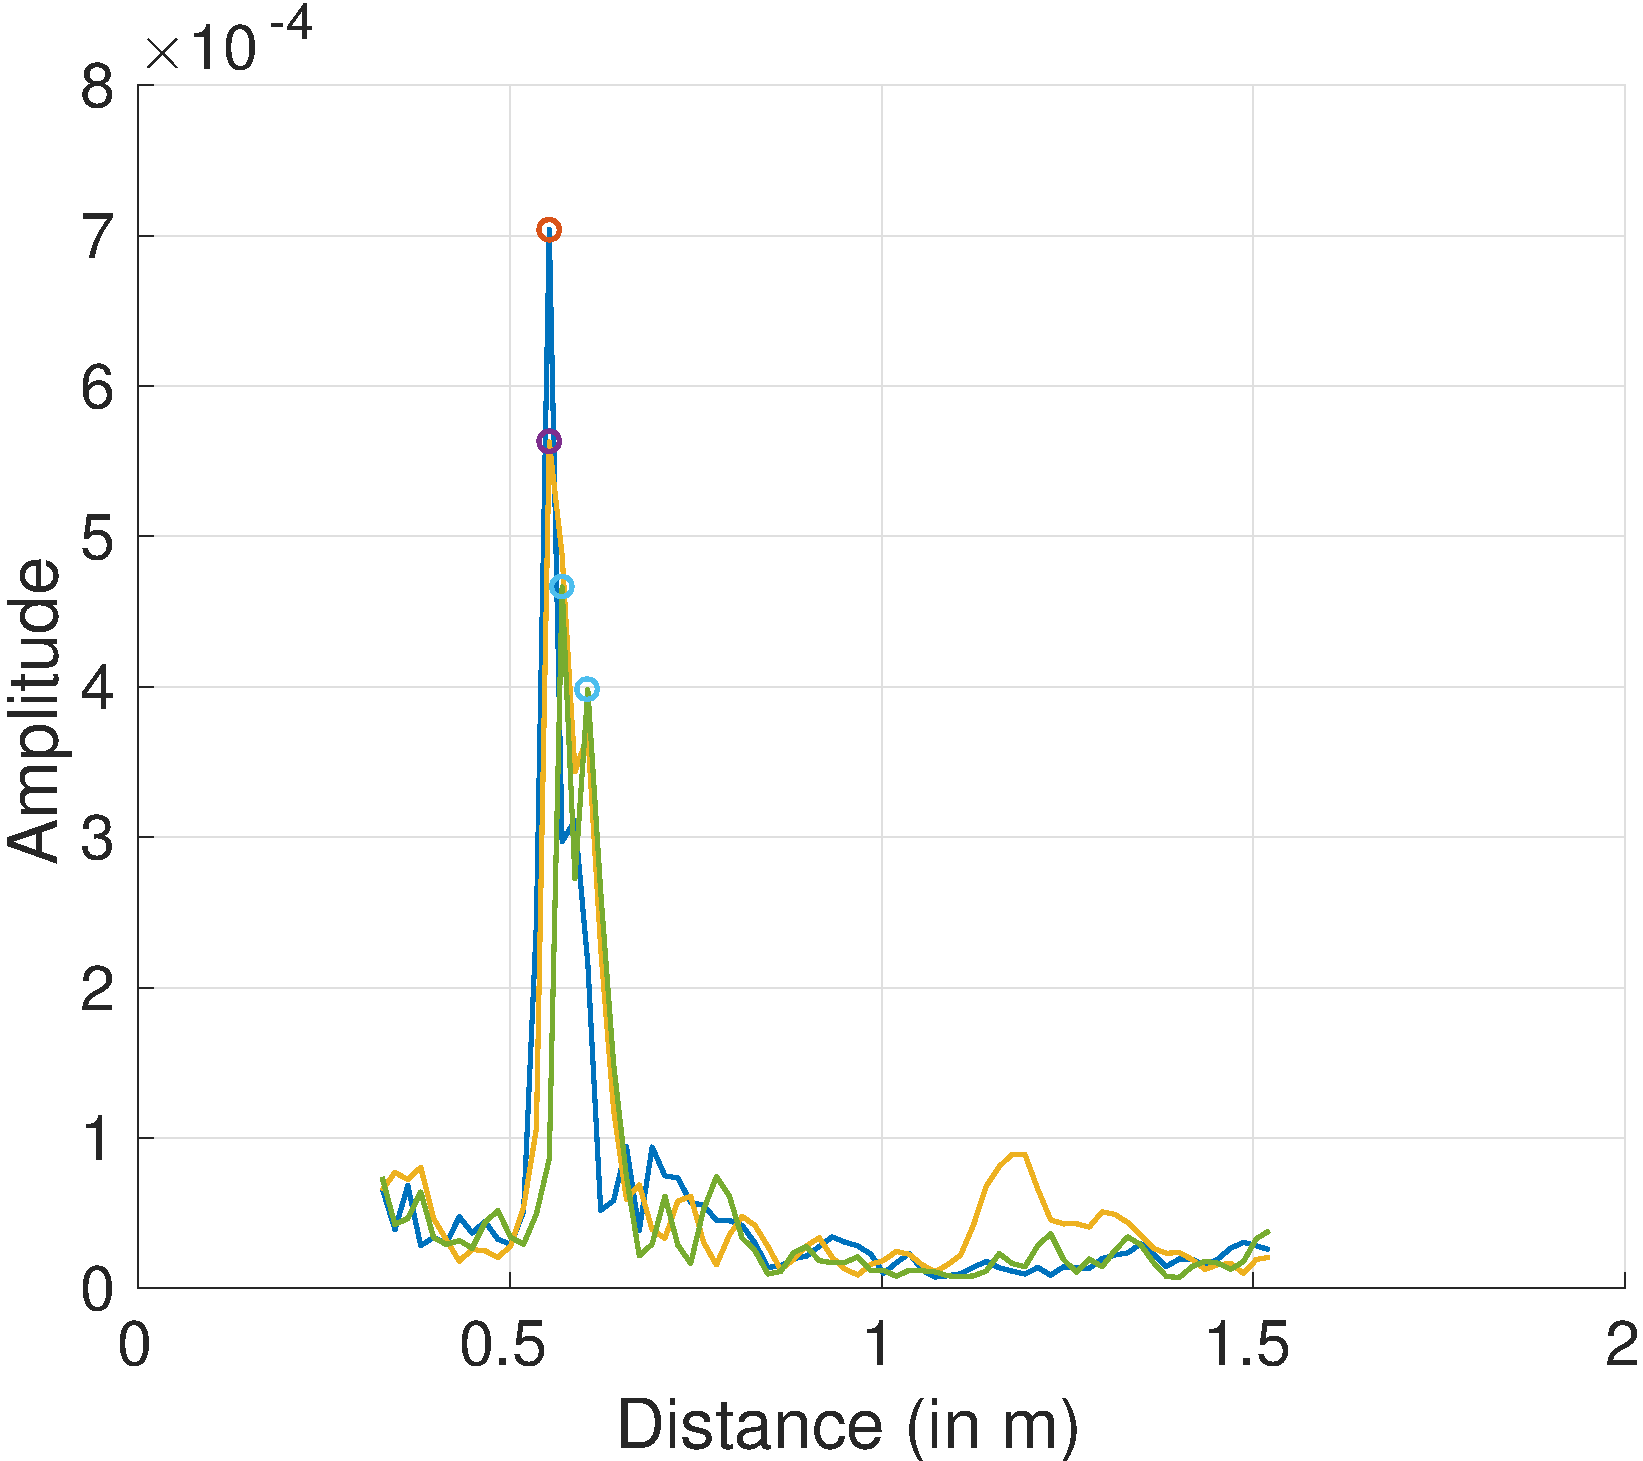
\includegraphics[width=\columnwidth]{figs/angle.pdf}
%\vspace{-0.1in}
\caption{{\small Perpendicular distance}}
%\vspace{-0.1in}
\label{fig:angle}
}
\end{figure}
\begin{itemize}
\item Junction causes mutliple peaks.
\item Maximum peak in FMCW corresponds to the main wall distance.
\item Always get perpendicular distance from wall.
\item Peak amplitude increases with the size of the reflector and it saturates after certain size.
\item Corner peaks are significantly different (at least for corner less than or equal to 90 degree). There are multiple peaks and peak spread is more.
\item Audio lobe direction and mic position matters.
\end{itemize}
